\section{Evaluation}\label{evaluation}

In this section, we present the evaluation result of Spark with SCache comparing with the original Spark. We first run simple DAG computing jobs with two stages to analyze the impact of shuffle pre-fetch on the scope of the hardware resources differences of the Spark cluster. The shuffle dependency between two stages contains one shuffle and two shuffles respectively. In addition, we run a shuffle heavy benchmark named Spark Terasort\cite{spark-tera}. In order to prove the performance gain of SCache with a real production workload -- Spark TPC-DS\cite{sparktpcds} and evaluate the improvement of SCache for each stage and the overall performance. At last, we prsent the overhead of sampling. Because a complex Spark application consists of multiple stages. The completion time of each stage varies under different input data and configurations, as well as different number of stages. This uncertainty leads to the dilemma that dramatic fluctuation in overall performance comparing. To present a straightforward illustration, we limit the scope of most evalutions in single stages. 

\subsection{Setup}\label{stepup}
We run our experiments on a 50 m4.xlarge nodes cluster on Amazon EC2\cite{aws}. Each node has 16GB memory and 4 CPUs. The network bandwidth is not specifically provided by Amazon. Our evaluation reveals the bandwidth is about 300 Mbps(see Figure \ref{fig:util}).

\subsection{Simple DAG Analysis}

\begin{figure*}
	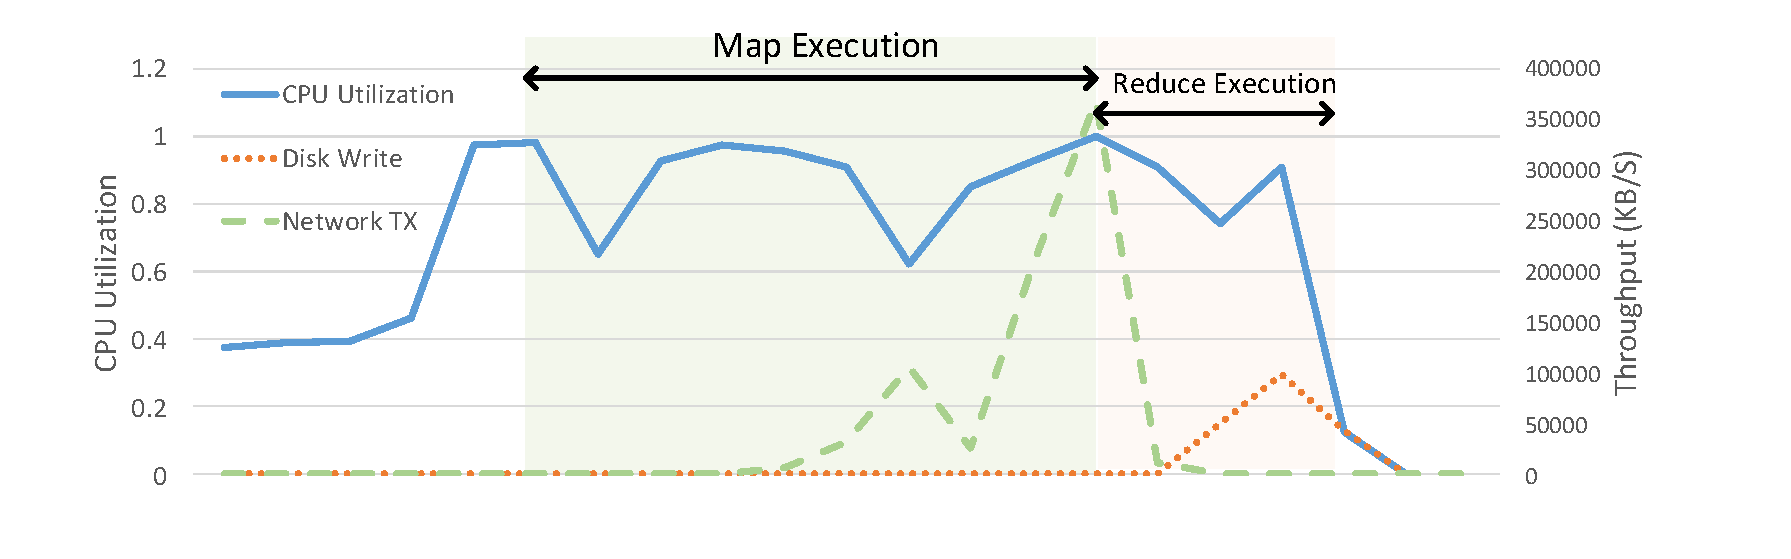
\includegraphics[width=\textwidth]{fig/scache_util}
	\caption{CPU utiliazation and I/O throughput of a node during a Spark single shuffle application With SCache}
	\label{fig:scache_util}
\end{figure*}

\subsubsection{Differential Runtime Hardware Utilization} 
We first run the same single shuffle test (GroupByTest from Spark example\cite{sparksource}) as we mentioned in Figure \ref{fig:util}. As shown in Figure \ref{fig:scache_util}, the hardware utilization is captured from one node during the job. Note that since the completion time of whole job is about 50\% less then Spark without SCache, the duration of Figure \ref{fig:scache_util} is cut in half as well. A overlap between CPU, disk and network can be easily obeserved in Figure \ref{fig:scache_util}. That is, the I/O operation will never cut off the computing process. By running Spark with SCache, the overall CPU utilization of the cluster stays in a high level. The decoupling of shuffle write from map tasks frees the CPU earlier, which leads to a faster map task computation. The shuffle pre-fetch starts the shuffle data transfer in the early stage of map phase shift the network transfer completion time, so that the computaion of reduce can start immediately afther scheduled. And this is the main performance gain we achieved on the scope of hardware utilization by SCache.

\subsubsection{Performace Gain in Detail}

As shown in \textcolor{red}{Figure}, we run these tow jobs with different input size in the cluster. We measure the completion time of each phase during the job, including shuffle write/read time and computing time. In the shuffle map stage, SCache optimizes \textcolor{red}{number} of shuffle write time. But time of shuffle write cannot be eliminate totally because the serialization is inevitable while moving data out of Java heap memory. Instead, the network transfer and disk read contribute significantly of decreasing time consumption of shuffle read, so that we can have a huge performance gain in both shuffle read and the completion time of whole reduce stage. By doing shuffle data pre-fetch, the shuffle read time decreases \textcolor{red}{number} on avarage, which contributes a \textcolor{red}{number} less completion time of reduce stages.

\subsection{Terasort}
In this part, we evaluate the both TeraSort\cite{spark-tera}. 

% \begin{figure}
% 	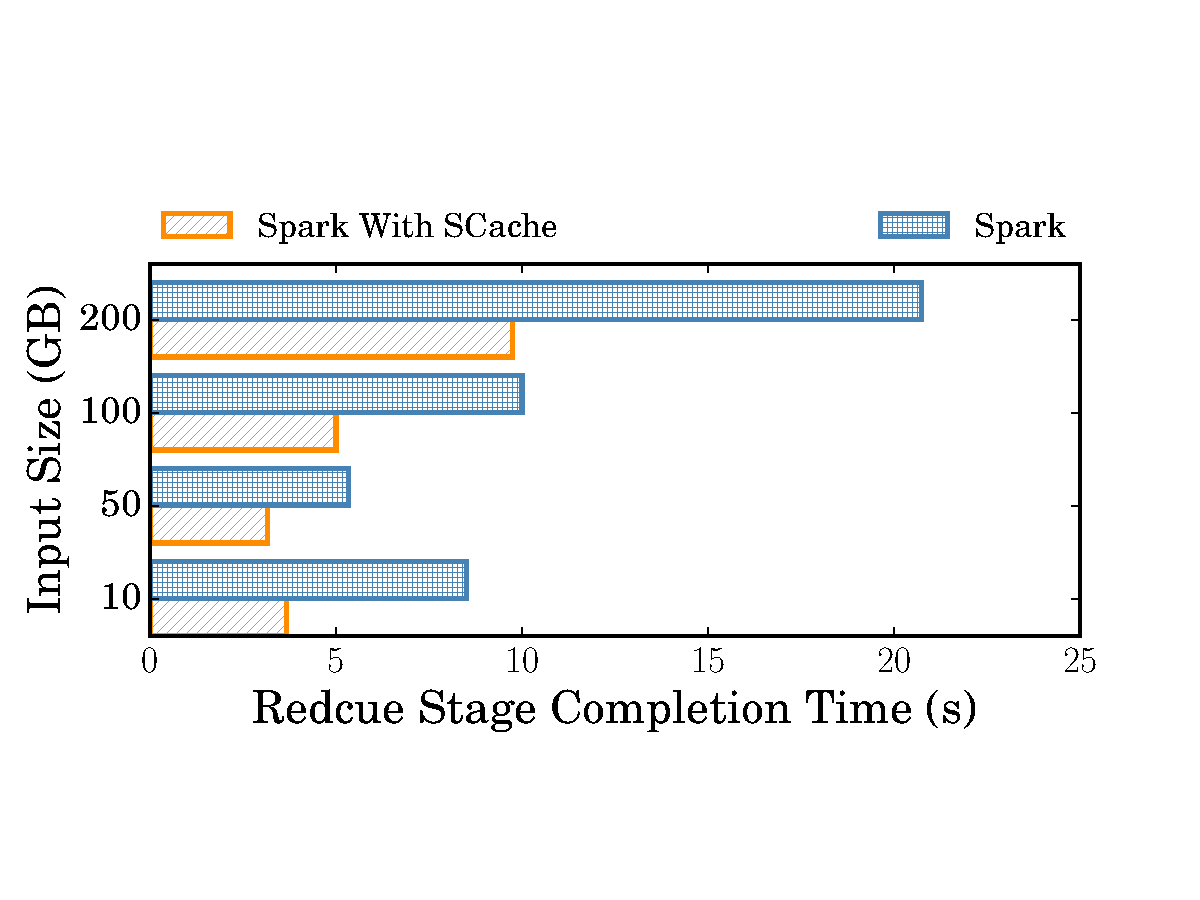
\includegraphics[width=\linewidth]{fig/tera}
% 	\caption{Reduce Stage Completion Time Comparsion}
% 	\label{fig:terasort}
% \end{figure}

% \begin{figure}
% 	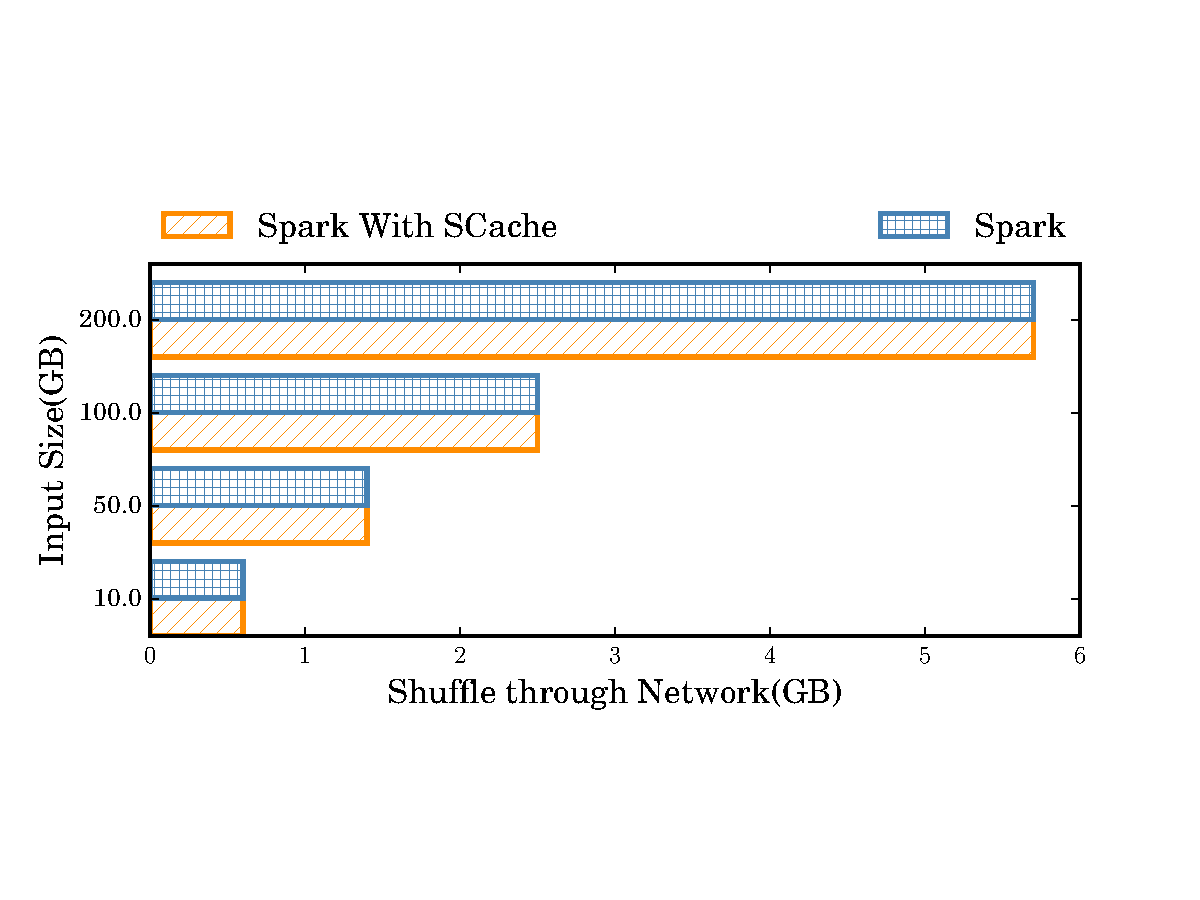
\includegraphics[width=\linewidth]{fig/tera_shuffle}
% 	\caption{Shuffle Data Size Comparsion}
% 	\label{fig:terashuffle}
% \end{figure}

\begin{figure}
\begin{subfigure}{\linewidth}
	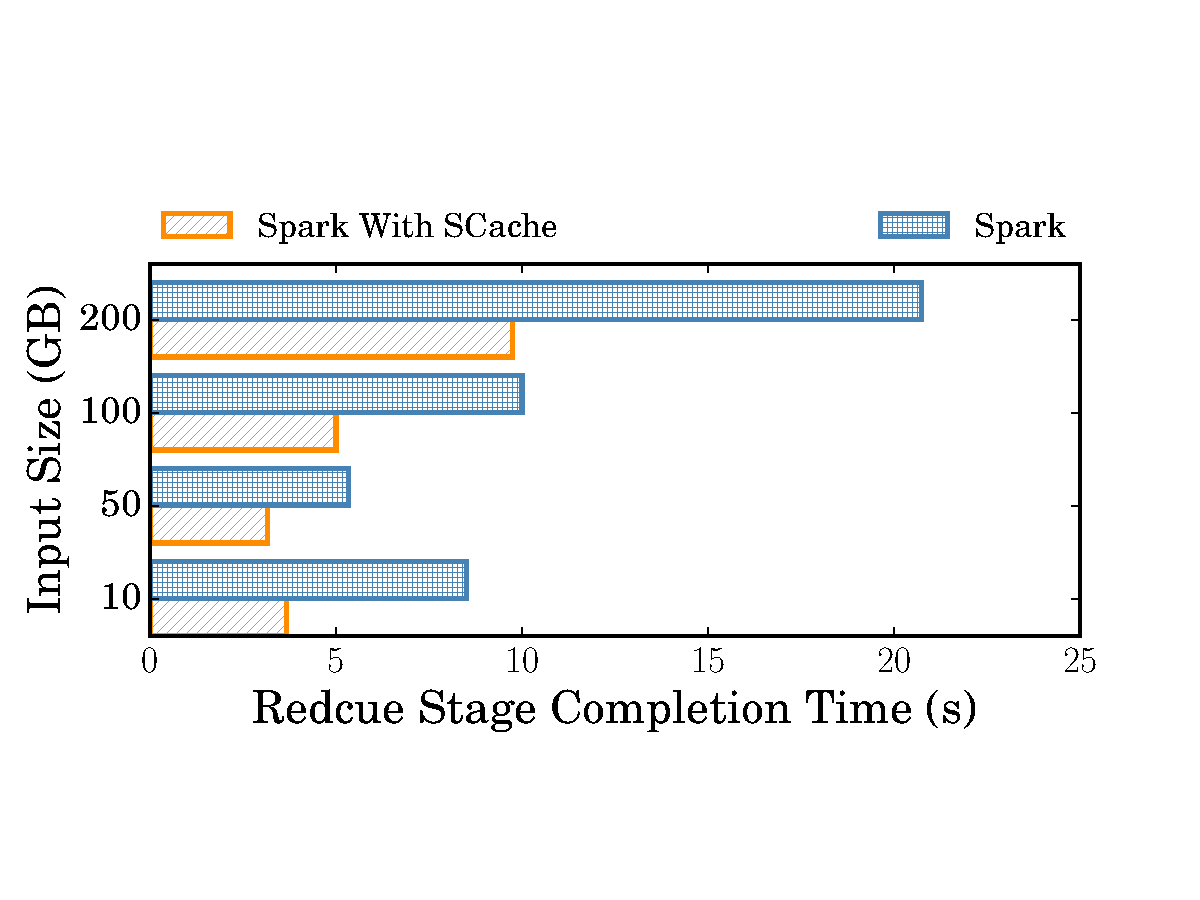
\includegraphics[width=\linewidth]{fig/tera}
	\caption{Reduce Stage Completion Time Comparsion}
	\label{fig:terasort}
\end{subfigure}
\begin{subfigure}{\linewidth}
	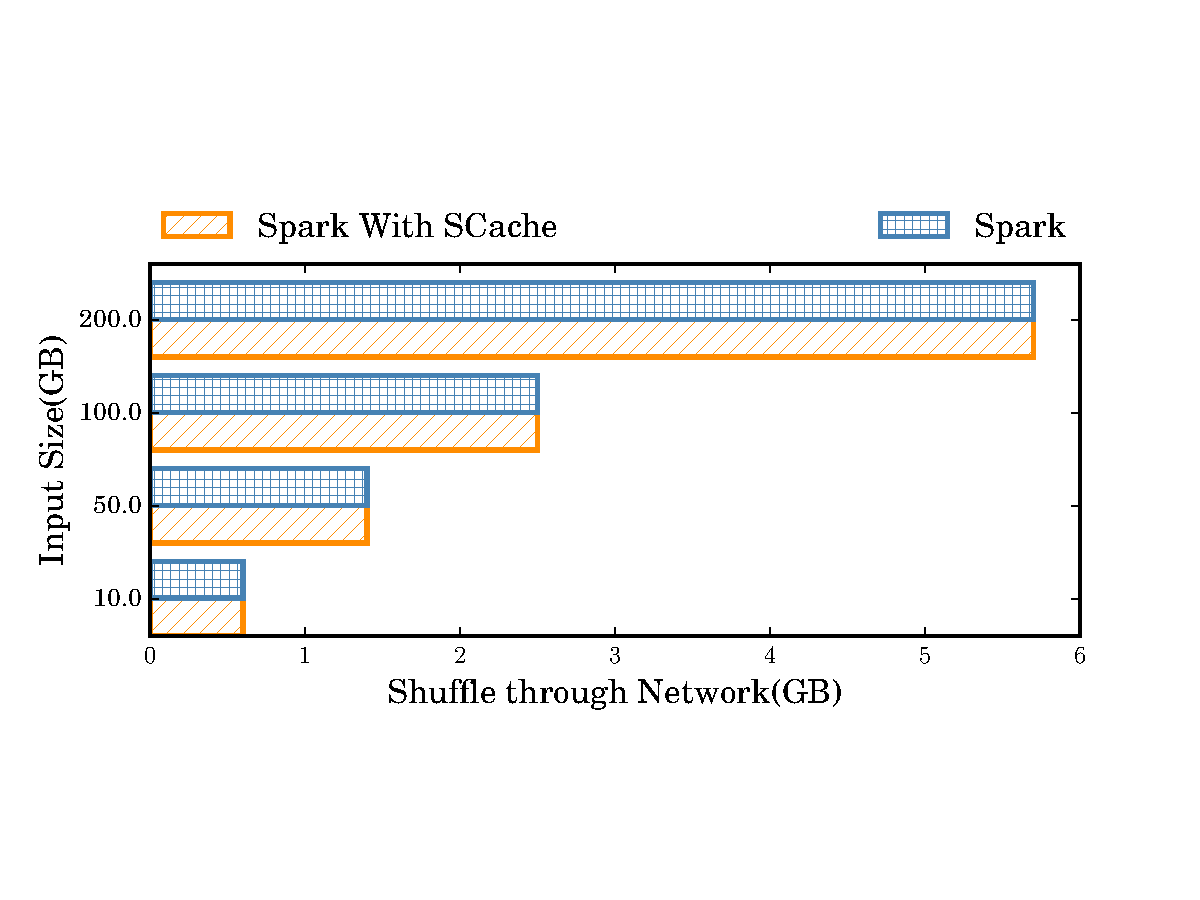
\includegraphics[width=\linewidth]{fig/tera_shuffle}
	\caption{Shuffle Data Size Comparsion}
	\label{fig:terashuffle}
\end{subfigure}
\caption{Terasort Evaluation}
\end{figure}

TeraSort is a shuffle intensive benchmark for distributed system analystics. As shown in Figure \ref{fig:terasort}, Spark with SCache runs 2 $\times$ faster during the reduce stage in a range from 10GB to 200GB input data. At the same time, the heuristic scheduling algorithms of SCache (Algorithm \ref{hminheap} and Algorithem \ref{mhminheap}) can obtain the exactly same scheduling result of reduce tasks, which decreases the network traffic. The result is presented in Figure \ref{fig:terashuffle}. In contrast, Spark delays scheduling reduce tasks the with the shuffle data locality to achieve this optimal.

\subsection{Production Workload}

We also evalute some shuffle heavy TPC-DS\cite{tpcds} on the cluster. TPC-DS benchmark is designed for modeling multiple users submitting varied queries (e.g. ad-hoc, interactive OLAP, data mining, etc.). TPC-DS contains 99 queries and is the considered as the  strandardized industry benchmark for testing big data systems. We evaluate performance of Spark with SCache by picking some of the TPC-DS queries with shuffle intensive attribute. As shown in Figure \ref{fig:tpcds}, on the horizon axis is query number, and on the vertical axis is query completion time. Spark with SCache outperforms the original Spark in almost all the queries in TPC-DS query set. Furthermore, in manyqueries, Spark with SCache outperforms original Spark by an order of magnitude. The overall reduction portion of query time that SCache achieved is 40\% on average. Since this evaluation presents the overall job compeletion time of queries, we believe that the optimization is promising.

\subsection{Overhead of Sampling}
In this part, we evaluate the overhead of sampling with different input data size and cluster scales. We uses the same Terasort\cite{spark-tera} for this evaluation. As shown in \textcolor{red}{Figure}, the overhead of sampling is very small comparing with the completion time of each stage.  \textcolor{red}{Figure} also prove that the overhead of sampling is stable with different number of nodes in cluster. It makes SCache a scalable system in cluster.

